\documentclass[12pt,a4paper,twoside,spanish]{article}      % Libro a 11 pt
\usepackage[height=17.5cm,width=13.5cm]{geometry}
\usepackage[spanish]{babel}         % diccionario
\usepackage[utf8]{inputenc}       % Acentos españoles
\usepackage{indentfirst}        % Siempre sangra
\usepackage{graphicx}           % Imagenes
\usepackage{epsfig}         % Graficos Postscript
\usepackage{tabularx}
\usepackage{sectsty}        
\usepackage{float}
\usepackage{geometry}	%Margenes del documento
\usepackage{caption}

\usepackage{color}
\usepackage[pdftex, colorlinks=true, linkcolor=blue, urlcolor=red, filecolor=magenta, citecolor=green]{hyperref}


\DeclareGraphicsExtensions{.png,.jpg,.mps}

%%%%%%%%%%%%%%%%%%%%%%%%%%%%%%%%%%%%%%%%%%%%%%%
%%%%%%%%%%%%%
%%%%%%%%%%%%% Margenes
%%%%%%%%%%%%%
%%%%%%%%%%%%%%%%%%%%%%%%%%%%%%%%%%%%%%%%%%%%%%%

\geometry{a4paper} % Tamaño y márgenes del documento
\geometry{left=2.5cm,top=2.5cm}
\geometry{bottom=2.5cm,right=2.5cm}

 % Estilo de los pies de figura/tabla
\captionsetup{format=hang,font=small,labelfont=bf}
\renewenvironment{abstract}{\list{}{\setlength{\leftmargin}{1cm}}{\setlength{
\rightmargin}{1cm}}\relax\item\ignorespaces\fontsize{12}{15}\selectfont {\bf \abstractname. }}{\unskip\endlist}%


%%%%%%%%%%%%%%%%%%%%%%%%%%%%%%%%%%%%%%%%%%%%%%%
%%%%%%%%%%%%%
%%%%%%%%%%%%% Profundidad de enumeracion y tabla de contenidos
%%%%%%%%%%%%%
%%%%%%%%%%%%%%%%%%%%%%%%%%%%%%%%%%%%%%%%%%%%%%%

\setcounter{secnumdepth}{3}
\setcounter{tocdepth}{3}


%%%%%%%%%%%%%%%%%%%%%%%%%%%%%%%%%%%%%%%%%%%%%%%
%%%%%%%%%%%%%
%%%%%%%%%%%%% Cuerpo del documento
%%%%%%%%%%%%%
%%%%%%%%%%%%%%%%%%%%%%%%%%%%%%%%%%%%%%%%%%%%%%%


\begin{document}

\def\chaptername{Capítulo}
\chapterfont{\LARGE\raggedleft}

%%%%%%%%%%%%%%%%%%%%%%%%%%%%%%%%%%%%%%%%%%%%%%%%%%%%%%%%%%%%%%%
%%%%%%%%%%%%%%%%%%%%%%%%%%%%%%%%%%%%%%%%%%%%%%%%%%%%%%%%%%%%%%%
% DISEÑO DE LA PAGINA DEL TITULO
%%%%%%%%%%%%%%%%%%%%%%%%%%%%%%%%%%%%%%%%%%%%%%%%%%%%%%%%%%%%%%%
%%%%%%%%%%%%%%%%%%%%%%%%%%%%%%%%%%%%%%%%%%%%%%%%%%%%%%%%%%%%%%%
\pagestyle{empty}

\begin{titlepage}
\setlength{\parindent}{0cm} \setlength{\parskip}{0cm}


\newcommand{\HRule}{\rule{\linewidth}{1mm}}

\vspace*{1.5cm}
\HRule \\[0.5cm]
\begin{center}
% Letra lineal y negrita
\textsf{\textbf{\Large SITIO WEB DE SUBASTAS \\[0.25cm] Práctica JAVA POJO Tapestry+Spring+Hibernate \\[0.5cm]}}
\HRule \vspace*{3cm}

\textsf{\textbf{\normalsize
Cedrón Santaeufemia, Francisco Abel\\
López Rivas, Nuria\\[4cm]
Integración de Sistemas\\
Área de Ingeniería Telemática\\ Universidad de A Coruña \\ Curso
2013/14}}
\end{center}
\end{titlepage}

\cleardoublepage

%%%%%%%%%%%%%%%%%%%%%%%%%%%%%%%%%%%%%%%%%%%%%%%
%%
%% TABLA DE CONTENIDOS
%%
%%%%%%%%%%%%%%%%%%%%%%%%%%%%%%%%%%%%%%%%%%%%%%%

\pagenumbering{Roman}
\tableofcontents
\cleardoublepage


%%%%%%%%%%%%%%%%%%%%%%%%%%%%%%%%%%%%%%%%%%%%%%%%%%%%%%%%%%%%%%%
%%%%%%%%%%%%%%%%%%%%%%%%%%%%%%%%%%%%%%%%%%%%%%%%%%%%%%%%%%%%%%%
%CONTENIDO DEL DOCUMENTO
%%%%%%%%%%%%%%%%%%%%%%%%%%%%%%%%%%%%%%%%%%%%%%%%%%%%%%%%%%%%%%%
%%%%%%%%%%%%%%%%%%%%%%%%%%%%%%%%%%%%%%%%%%%%%%%%%%%%%%%%%%%%%%%

%numeros arábigos
\pagenumbering{arabic} \pagestyle{myheadings}

%indentaciones y espaciado entre párrafos
\setlength{\parindent}{1,5cm} \setlength{\parskip}{0,7cm}


%%%%%%%%%%%%%%%%%%%%%%%%%%%%%%%%%%%%%%%%%%%%%%%%%%%%%%%%%%%%%%%%%%%%%%%%%%%%%%%
\section{Arquitectura global.}
%%%%%%%%%%%%%%%%%%%%%%%%%%%%%%%%%%%%%%%%%%%%%%%%%%%%%%%%%%%%%%%%%%%%%%%%%%%%%%%
A continuación se muestan los principales paquetes del diseño.
\begin{figure}[H]
  \centering
    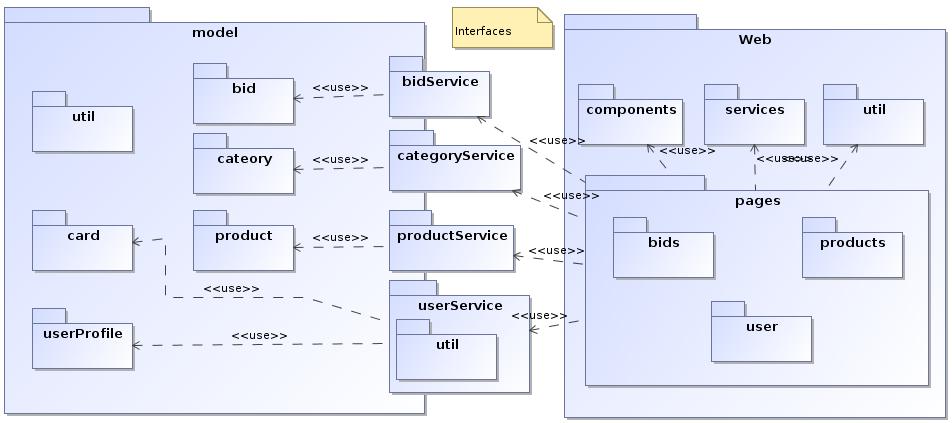
\includegraphics[width=1\textwidth]{paquetes}
  \caption{Paquetes del diseño.}
  \label{fig:packages}
\end{figure}

Describiendo brevemente la función de cada uno de los paquetes:
\begin{enumerate}
 \item \textbf{model}: Paquete principal de la capa modelo y contenedor de los demás paquetes. Los paquete situados ligeramente
 fuera del paquete principal, correspondientes a los servicios, actúan como interfaces entre ambos paquetes generales. Cada
 entidad persistente dispone de su propio paquete, el cual contiene los DAO's para interactuar con la base de datos.\\
  La mayoría de los paquetes son autodescriptivos mediante su nombre. El paquete \textit{util} contiene el fichero 
\textit{GlobalNames}, el cual define la ruta al fichero de configuración de Spring.
 \item \textbf{web}: Paquete principal de la capa web que contiene los siguientes paquetes:
  \begin{itemize}
   \item components: Para los elementos comunes de las páginas.
   \item services: Contiene las politicas y los filtros que se utilizan en la aplicación web.
   \item util: Contiene ficheros para la definición de la sesión del usuario, el uso de cookies y las configuraciones para el
   uso de tablas, paginación y listados en los \textit{.tml}.
   \item pages: Contiene los paquetes que implementan las páginas que se muetran al usuario.
    \begin{itemize}
     \item bids: Control del formulario de apuestas.
     \item products: Control para listar productos, mostrar sus detalles y del formulario para añadirlos.
     \item user: Control de los formularios de registro, autenticación, cambio de contraseña, añadir una tarjeta o modificarla y
     modificar los datos de registro. Además contiene una página que muestra todos los datos del usuario que se puedan visualizar.
    \end{itemize}
  \end{itemize}
\end{enumerate}



%%%%%%%%%%%%%%%%%%%%%%%%%%%%%%%%%%%%%%%%%%%%%%%%%%%%%%%%%%%%%%%%%%%%%%%%%%%%%%%
\section{Modelo.}
%%%%%%%%%%%%%%%%%%%%%%%%%%%%%%%%%%%%%%%%%%%%%%%%%%%%%%%%%%%%%%%%%%%%%%%%%%%%%%%

%%%%%%%%%%%%%%%%%%%%%%%%%%%%%%%%%%%%%%%%%%%%%%%%%%%%%%%%%%%%%%%%%%%%%%%%%%%%%%%
\subsection{Clases persistentes.}
%%%%%%%%%%%%%%%%%%%%%%%%%%%%%%%%%%%%%%%%%%%%%%%%%%%%%%%%%%%%%%%%%%%%%%%%%%%%%%%

\begin{figure}[H]
  \centering
    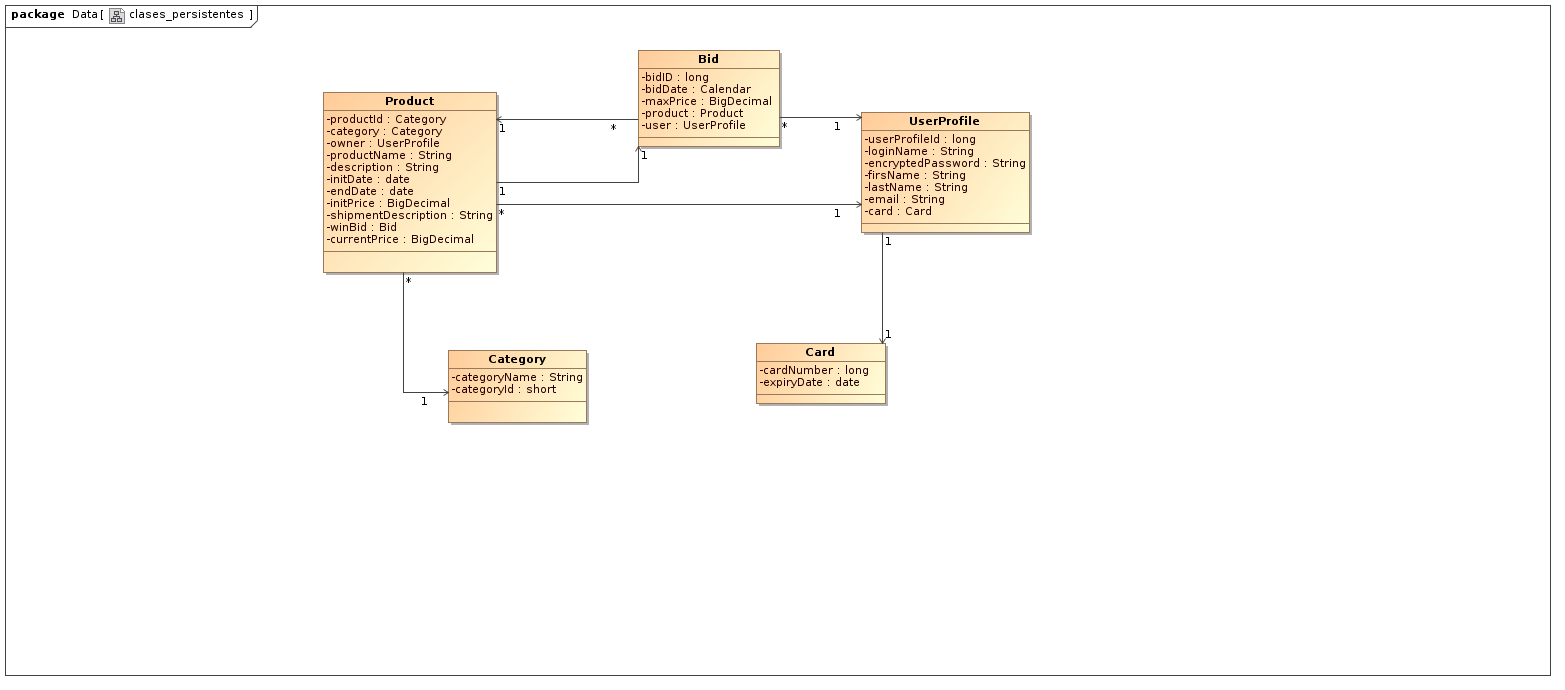
\includegraphics[width=1\textwidth]{clases_persistentes}
  \caption{Clases persistentes.}
  \label{fig:Clases_persistentes}
\end{figure}

%%%%%%%%%%%%%%%%%%%%%%%%%%%%%%%%%%%%%%%%%%%%%%%%%%%%%%%%%%%%%%%%%%%%%%%%%%%%%%%
\subsection{Interfaces de los servicios ofrecidos por el modelo.}
%%%%%%%%%%%%%%%%%%%%%%%%%%%%%%%%%%%%%%%%%%%%%%%%%%%%%%%%%%%%%%%%%%%%%%%%%%%%%%%

\begin{figure}[H]
  \centering
    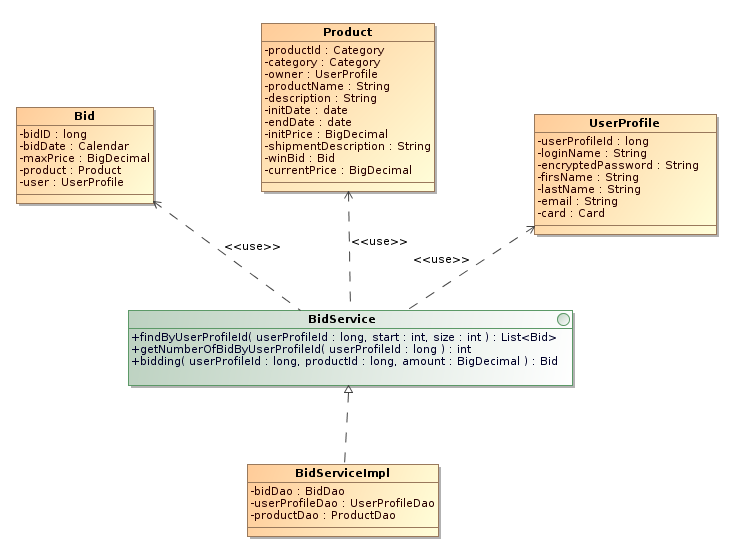
\includegraphics[width=1\textwidth]{BidService}
  \caption{Interfaz del servicio de apuestas.}
  \label{fig:BidService}
\end{figure}

\begin{figure}[H]
  \centering
    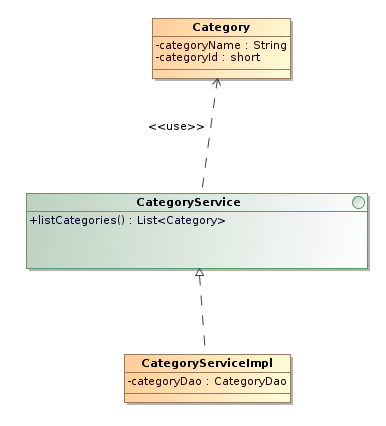
\includegraphics[scale=0.9]{CategoryService}
  \caption{Interfaz del servicio de categoría.}
  \label{fig:CategoryService}
\end{figure}

\begin{figure}[H]
  \centering
    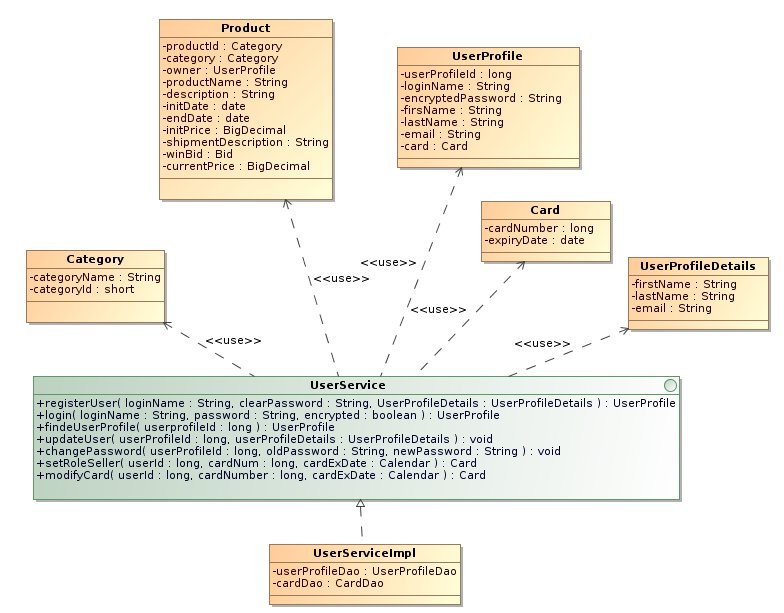
\includegraphics[scale=0.8]{user_service}
  \caption{Interfaz del servicio de usuario.}
  \label{fig:UserService}
\end{figure}

\begin{figure}[H]
    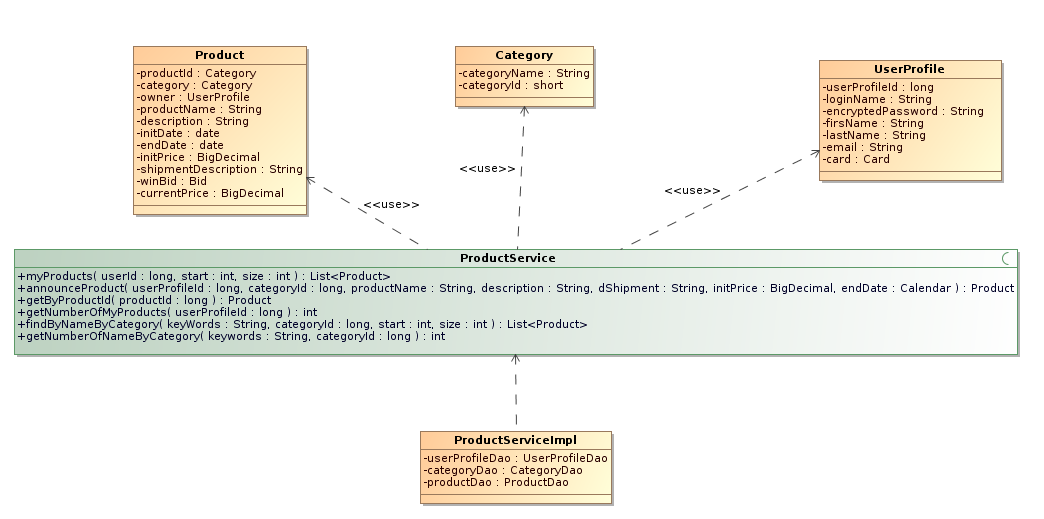
\includegraphics[angle=90,scale=0.8]{ProductService}
  \caption{Interfaz del servicio de productos.}
  \label{fig:ProductService}
\end{figure}

La interfaz lógica de \textit{card} no fue creada ya que su funcionalidad se incluye dentro de la interfaz de \textit{userService}.
De las otras 4 interfaces podemos decir:
\begin{itemize}
 \item bidService permite la búsqueda de las pujas de un usuario y la funcionalidad para realizar la propia puja.
 \item categoryService otorga acceso a la lista de categorías.
 \item productService permite buscar productos por palabra clave o por categoría. También implementa la lógica para añadir productos.
 \item userService trata todo lo relacionado con los datos del usuario, incluyendo la creación de una tarjeta de crédito.
\end{itemize}

%%%%%%%%%%%%%%%%%%%%%%%%%%%%%%%%%%%%%%%%%%%%%%%%%%%%%%%%%%%%%%%%%%%%%%%%%%%%%%%
\section{Interfaz gráfica.}
%%%%%%%%%%%%%%%%%%%%%%%%%%%%%%%%%%%%%%%%%%%%%%%%%%%%%%%%%%%%%%%%%%%%%%%%%%%%%%%
La interfaz gráfica consta de una capa común (Layout) y una serie de páginas que se explican a continuación.


La página inicial consta de una barra de búsqueda, ya que se pueden ver los productos disponibles para pujar tanto si se está
autenticado como si no.

\begin{figure}[H]
  \centering
    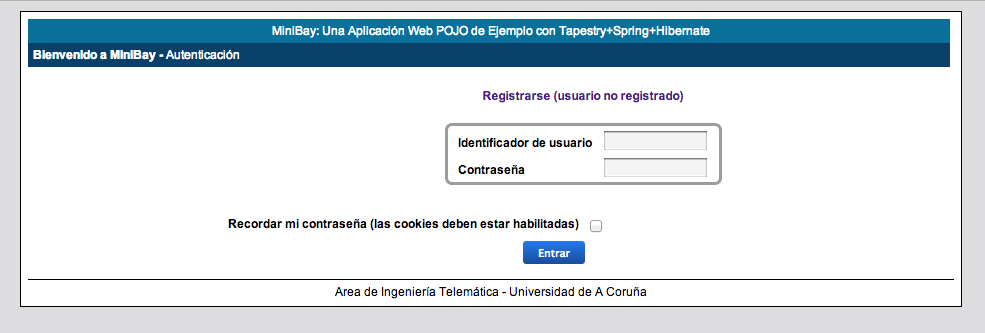
\includegraphics[width=1\textwidth]{autenticacion.png}
  \caption{Formulario de autenticación.}
  \label{fig:Autenticacion}
\end{figure}

Para poder pujar es necesario estar autenticado, a esto se llega pulsando en el enlace ``Autenticar'' en la barra de menú. En
caso de no estar registrado, en la misma página de autenticación hay un enlace que lleva a una pagína de registro.

Una vez autenticado, se accede a la página principal.
\begin{figure}[H]
  \centering
    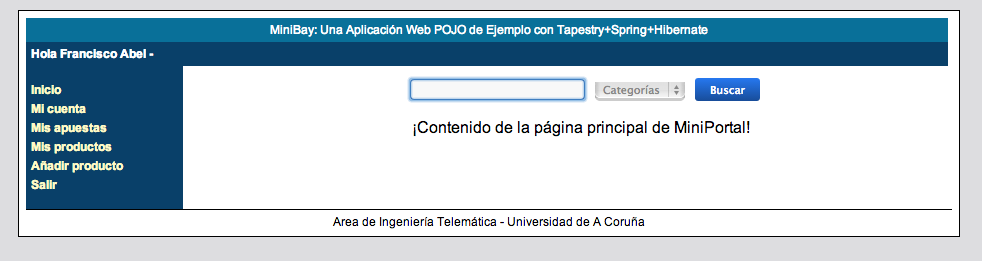
\includegraphics[width=1\textwidth]{pagina_principal.png}
  \caption{Página principal.}
  \label{fig:Principal}
\end{figure}

En la parte izquierda de la \ref{fig:Principal} pueden verse una serie de enlaces a los distintos servicios de la página. El primero de ellos es un enlace a la misma página que se muestra en dicha imagen, siendo útil cuando se quiere volver ahí desde cualquiera de las otras páginas.


El segundo enlace lleva a una página con diferentes tipos de información del usuario.

\begin{figure}[H]
  \centering
    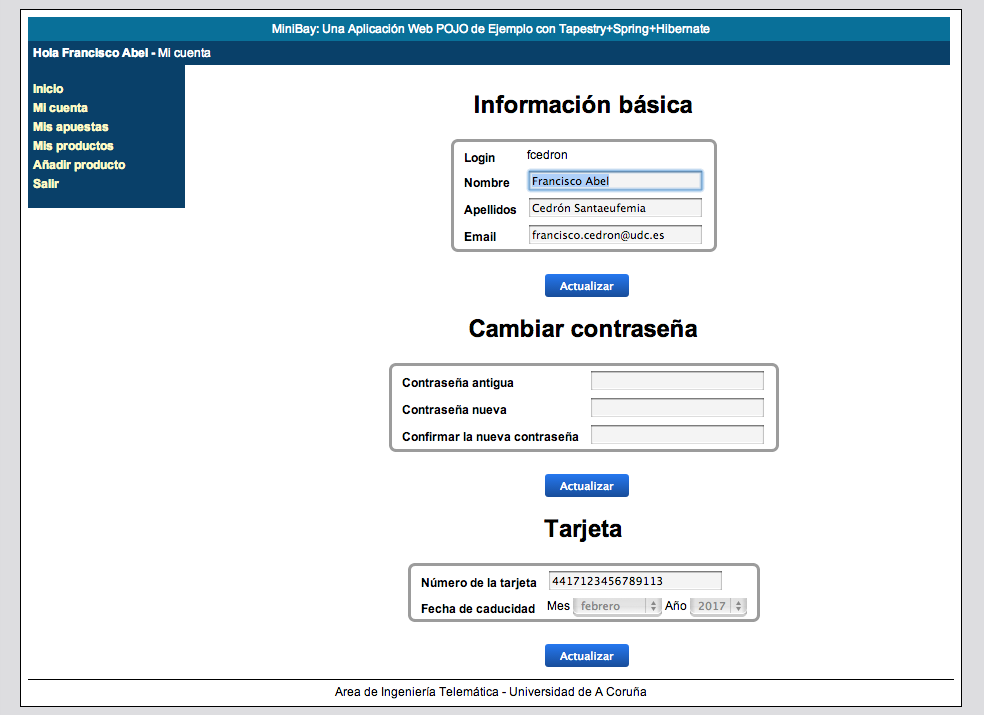
\includegraphics[width=1\textwidth]{mi_cuenta.png}
  \caption{Cuenta personal del usuario.}
  \label{fig:myaccount}
\end{figure}

En la \ref{fig:myaccount} pueden verse 3 formularios. El primero de ellos muestra la información del usuario, y al mismo tiempo
permite modificarla, escribiendo el nuevo valor en el campo que se desee cambiar y pulsando en ``Actualizar''.

El segundo formulario sirve para cambiar la contraseña de acceso al sitio. Por último, el tercero muestra los datos de la 
tarjeta de crédito propiedad del usuario, y de igual forma que con la información personal, también se pueden modificar estos
valores. En caso de que el usuario no haya añadido ninguna tarjeta los campos se mostrarán en blanco, y deberán ser rellenados
para añadir una.

El motivo de tener estos 3 formularios aquí es mantener el número de página al mínimo.

El tercer enlace de la figura \ref{fig:Principal} lleva a un listado de las apuestas realizadas por el usuario.

\begin{figure}[H]
  \centering
    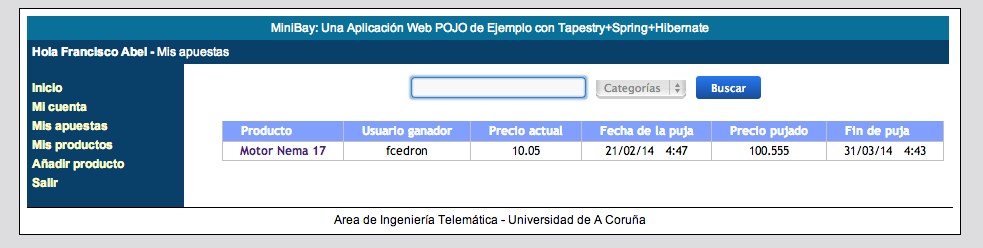
\includegraphics[width=1\textwidth]{mis_apuestas.png}
  \caption{Apuestas realizadas por el usuario.}
  \label{fig:mybids}
\end{figure}

Los únicos datos que se muestran aquí son: el nombre del producto, el propietario del producto, la fecha en que se realizó
la puja y la cantidad pujada. El nombre del producto es a su vez un enlace a otr página que contiene una descripción más en
detalle de dicho producto.

\begin{figure}[H]
  \centering
    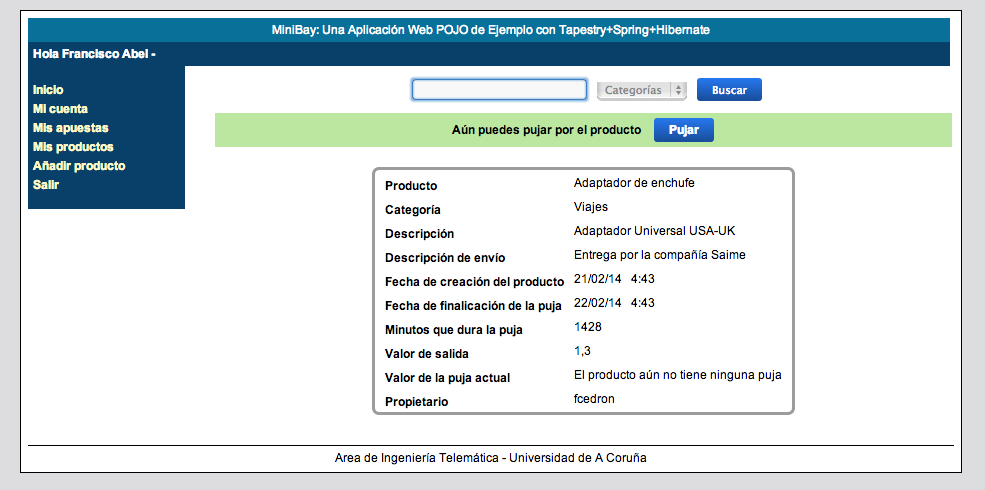
\includegraphics[width=1\textwidth]{detalles2.png}
  \caption{Detalles de un producto.}
  \label{fig:productDetails}
\end{figure}

Como puede observarse en la figura \ref{fig:productDetails} esta página contiene un botón que permite al usuario pujar por el
producto que está consultando, además de informales si va ganando o no la puja, y aumentar el valor de ésta si así lo desea.

\begin{figure}[H]
  \centering
    
\includegraphics[width=0.6\textwidth]{puja_ganadora.png}
  \caption{Información sobre la puja.}
  \label{fig:winBid}
\end{figure}

El siguiente enlace, siguiendo el orden, lleva a un listado de los productos añadidos por el usuario.

\begin{figure}[H]
  \centering
    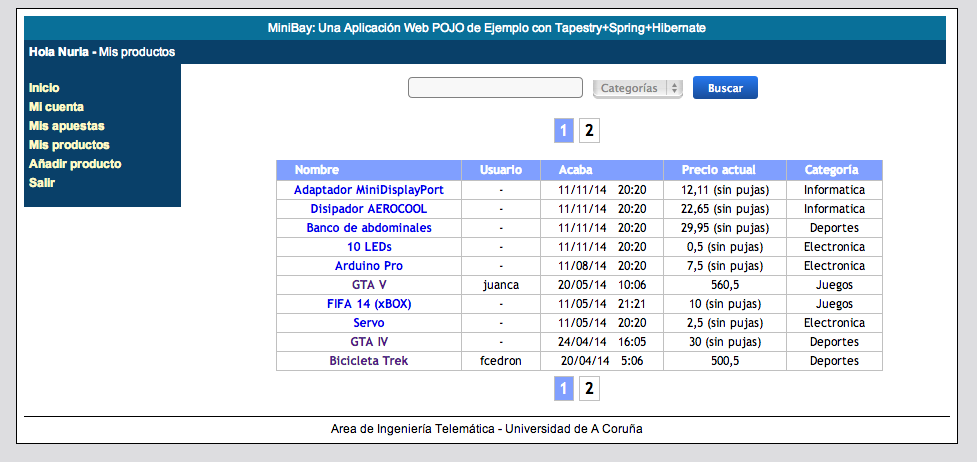
\includegraphics[width=1\textwidth]{mis_productos.png}
  \caption{Productos del usuario.}
  \label{fig:myProducts}
\end{figure}

Los detalles que se muestran aquí son: nombre del producto, propietario del producto, fecha y hora de finalización de la puja,
valor actual en el proceso de puja y la categoría a la que pertenece. Al igual que en el caso del listado de apuestas, el nombre
del producto es un enlace a la página mostrada en la figura \ref{fig:productDetails}. En el apartado del valor actual del
producto también se muestra si se ha hecho alguna puja por él.

El penúltimo enlace lleva a un formulario para que el usuario pueda añadir productos.

\begin{figure}[H]
  \centering
    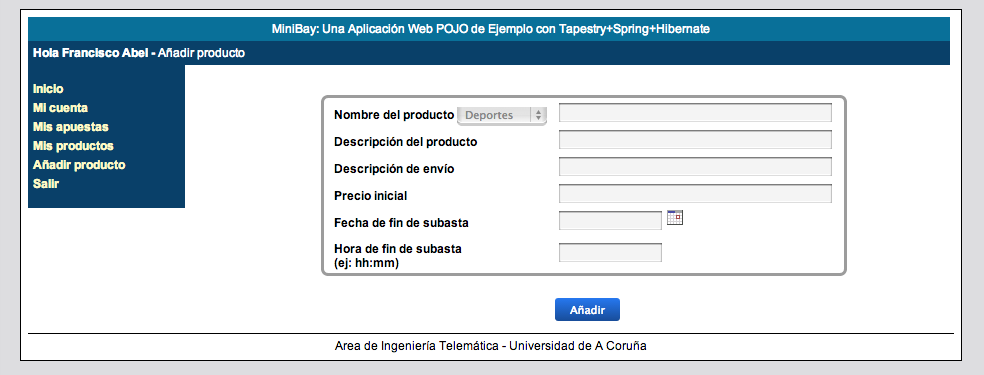
\includegraphics[width=1\textwidth]{anadir_producto.png}
  \caption{Formulario para añadir productos.}
  \label{fig:addProduct}
\end{figure}

Todo los campos son obligatorios. Una vez añadido el producto, se redirige a la página con sus detalles.

El último enlace cumple la función de ``logout'', cerrando la sesión en el sitio.
%%%%%%%%%%%%%%%%%%%%%%%%%%%%%%%%%%%%%%%%%%%%%%%%%%%%%%%%%%%%%%%%%%%%%%%%%%%%%%%
\section{Servicios XML.}
%%%%%%%%%%%%%%%%%%%%%%%%%%%%%%%%%%%%%%%%%%%%%%%%%%%%%%%%%%%%%%%%%%%%%%%%%%%%%%%
Los formatos de la URL's de los servicios XML son los siguiente:

\begin{enumerate}
 \item Información detallada de un producto: \\
    \textcolor{red}{http://localhost:8080/minibay/products/xmlproductdetails?productid=X}\\
    X representa el id del producto del cual se quieren ver los detalles.\\
    El formato de salida consta de una etiqueta con los atributos correspondientes a los detalles del producto. Obviando los
    autodescriptivos, el significado es el siguiente:
    \begin{itemize}
     \item initDate: Fecha de creación del producto.
     \item endDate: Fecha de fin de subasta.
     \item initPrice: Precio que pone inicialmente el anunciante del producto.
     \item dShipment: Descripción del envío del producto.
     \item currentPrice: Valor actual del producto. Varía según se vayan haciendo pujas.
     \item winBid: Usuario que va ganando la subasta.
    \end{itemize}
\begin{verbatim}
 <product xmlns:t="http://tapestry.apache.org/schema/tapestry_5_3.xsd"
		  xmlns:p="tapestry:parameter">
	<t:if test="product">
	      name=${product.productName}
	      category=${product.category.categoryName}
	      owner=${product.owner.loginName}
	      initDate=${product.initDate.time}
	      endDate=${product.endDate.time}
	      description=${product.description}
	      initPrice=${product.initPrice}
	      dShipment=${product.shipmentDescription}
	      currentPrice=${product.currentPrice}
	      <t:if test="product.winBid">
		      winBid=${product.winBid.user.loginName}
	      </t:if>
	    <p:else>
		    <errorNoProduct />
	    </p:else>
    </t:if>
</product>
\end{verbatim}


    
  \item Búsqueda de productos por palabra clave del nombre:\\ 
      \textcolor{red}{http://localhost:8080/minibay/products/XmlListProducts?start=X\&size=Y\&keywords=Z}\\
    X representa en qué producto se comienza a listar.\\
    Y representa cuántos productos se listarán por página.\\
    Z representa las palabras clave mediante las que se va a realizar la búsqueda.\\
    El formato de salida consta de una única etiqueta que contiene los atributos relevantes del producto mostrado. Habrá una línea
    por cada producto en la lista.
\end{enumerate}

\begin{verbatim}
     <products total="${total}" show="${show}" 
      xmlns:t="http://tapestry.apache.org/schema/tapestry_5_3.xsd">
	<t:loop t:source="list" t:value="Product">
        <product
        	id="${product.productId}"
        	category="${product.category.categoryName}"
        	name="${product.productName}"
        	seller="${product.owner.loginName}"
        	ends="${endDate}"
        	minutesToEnd="${minutesToend}"
        	price="${price}"
        	/>
    </t:loop>
</products> 
\end{verbatim}



%%%%%%%%%%%%%%%%%%%%%%%%%%%%%%%%%%%%%%%%%%%%%%%%%%%%%%%%%%%%%%%%%%%%%%%%%%%%%%%
\section{Partes opcionales.}
%%%%%%%%%%%%%%%%%%%%%%%%%%%%%%%%%%%%%%%%%%%%%%%%%%%%%%%%%%%%%%%%%%%%%%%%%%%%%%%

%%%%%%%%%%%%%%%%%%%%%%%%%%%%%%%%%%%%%%%%%%%%%%%%%%%%%%%%%%%%%%%%%%%%%%%%%%%%%%%
\subsection{Implementación de AJAX.}
%%%%%%%%%%%%%%%%%%%%%%%%%%%%%%%%%%%%%%%%%%%%%%%%%%%%%%%%%%%%%%%%%%%%%%%%%%%%%%%
En este apartado explicaremos como se ha realizado la parte de optativa que se corresponde con AJAX.

Hemos decidido implementar la funcionalidad de AJAX en la página que muestra los detalles del usuario, la cual se muestra en la figura \ref{fig:myaccount}.
El motivo de insertarlo aquí fueron los formularios. Si un usuario comete un error en la modificación de alguno de los datos, por ejemplo, si en un cambio de
contraseña, al reescribirla no coincide con la primera inserción, o si escribe mal la vieja. En estos casos se usa AJAX para que se muestre el mensaje de error
sin necesidad de recargar la página entera.

Además de esto, si se modifican correctamente cualquiera de los datos presentes, solo se recargará el formulario afectado. El siguiente código muestra la 
implementación de estos casos.

\begin{verbatim}
Object onSuccessFromChangeCard() {
	okCard = messages.get("ok-card");
	return request.isXHR() ? zoneFormCard.getBody() : null;
}

Object onFailureFromChangeCard() {
	return request.isXHR() ? zoneFormCard.getBody() : null;
}
    

Object onSuccessFromChangePassword() {
	CookiesManager.removeCookies(cookies);
	okPassword = messages.get("ok-pass");
	return request.isXHR() ? zoneFormPassword.getBody() : null;
}
    
Object onFailureFromChangePassword() {
	return request.isXHR() ? zoneFormPassword.getBody() : null;
}
    
Object onSuccessFromChangeInfo() throws InstanceNotFoundException {
	userService.updateUserProfileDetails(
		userSession.getUserProfileId(), new UserProfileDetails(
		firstName, lastName, email));
	userSession.setFirstName(firstName);
	okInfo = messages.get("ok-info");
	return request.isXHR() ? zoneFormInfo.getBody() : null;
}
      
Object onFailureFromChangeInfo() {
	return request.isXHR() ? zoneFormInfo.getBody() : null;
}
\end{verbatim}

Para utilizar esas funciones fue necesario injectar los componentes ``Zone'' y ``Request'' e incorporar los siguientes paquetes al fichero 
``MyAccount.java'':
\begin{verbatim}
    import org.apache.tapestry5.corelib.components.Zone;
    import org.apache.tapestry5.services.Request;
 
    @InjectComponent
    private Zone zoneFormCard;
 
    @InjectComponent
    private Zone zoneFormPassword;
 
    @InjectComponent
    private Zone zoneFormInfo;
    
    @Inject
    private Request request;
\end{verbatim}

Podemos definir:\\
\textbf{Zone}: Las ``Zone'' definen el área de datos actualizable, corresponden a un bloque de la plantilla tml.\\
\textbf{Request}: Permite controlar la petición http para saber si se trata de AJAX.

En los .tml se hicieron los siguientes cambios:
\begin{verbatim}
	<t:zone t:id="zoneFormInfo" id="zoneFormInfo">
		<form t:type="Form" t:id="changeInfo" t:zone="^">
		
	<t:zone t:id="zoneFormPassword" id="zoneFormPassword">
		<form t:type="Form" t:id="changePassword" t:zone="^">
	
	<t:zone t:id="zoneFormCard" id="zoneFormCard">
		<form t:id="changeCard" t:type="form" t:zone="^">
\end{verbatim}

Con eso definimos las zonas que se modificarán dinámicamente.

Este proceso también se definió para el formulario de añadir productos, dando lugar a código similar.

Además de lo anterior, también se añadió una parte de AJAX al utilizar el componente ``GridDataSource'' para definir las listas de productos y pujas.

En caso de que un usuario no disponga de JavaScript en su navegador, se añadió un aviso en Layout.tml
\begin{verbatim}
 <noscript class="js-required">
	<p class="t-red">
       ${message:javascript_required}
    </p>
</noscript>
\end{verbatim}




\subsection{Pruebas funcionales contra la interfaz Web.}

	Las pruebas funcionales contra la interfaz Web son pruebas que comprueban el correcto funcionamiento de una aplicación Web usando directamente su interfaz Web. Se han implementado dos casos de prueba, los cuales se corresponden con dos secuencias de navegación que representan las funcionalidades que la aplicación ofrece al usuario. Los casos de prueba implementados son:
\begin{itemize}
	\item Registro, cambio de contraseña y autenticación con la nueva contraseña.
	\item Realizar una apuesta sobre un producto concreto.
\end{itemize}

	La implementación de estos dos casos de prueba se ha realizado en un nuevo proyecto. La razón por lo que se ha hecho así es porque en el otro proyecto están los test de la capa modelo que se ejecutan con más frecuencia, mientras que los test contra la interfaz no están en ese caso y tardan bastante más es llevarse a cabo. De hecho, si este tipo de test contra la interfaz Web fuese muy numeroso, incluso podría ser inviable ejecutarlos con la frecuencia necesaria.
	
	Para la implementación de los test automáticos de la interfaz web se ha utilizado el componente \textit{WebDriver} de la herramienta \textit{Selenium} junto con JUnit. Estas herramientas abren automáticamente un navegador para ejecutar cada caso de prueba, es decir, ejecutan la secuencia de navegación del caso de prueba y jacen las comprobaciones necesarias para verificar el correcto funcionamiento de la aplicación.
	
A continuación se detalla la secuencia de navegación realizada en cada caso de prueba.

\subsubsection{Registro, cambio de contraseña y autenticación con la nueva contraseña.}

La secuencia de navegación utilizada para llevar a cabo el caso de prueba es la siguiente:
\begin{enumerate}
	\item Acceder a la página principal de la aplicación.
	\item Hacer clic en el enlace ``Autenticarse''.
	\item Hacer clic en el enlace ``Registrarse (usuario no registrado)''.
	\item Cubrir el formulario de registro.
	\item Hacer clic en el botón de ``Registrar''.
	\item Hacer clic en el enlace ``Mi cuenta''.
	\item Rellenar el formulario destinado para cambiar la contraseña.
	\item Hacer clic en el botón de``Actualizar''.
	\item Hacer clic en el enlace ``Salir''.
	\item Hacer clic en el enlace ``Autenticarse''.
	\item Cubrir el formulario de inicio de sesión.
	\item Hacer clic en el botón de ``Entrar''.	
\end{enumerate}

\subsection{Realizar una apuesta sobre un producto concreto.}

	Para llevar a cabo esta prueba se usarán los datos que hay en el proyecto de las pruebas funcionales contra la interfaz web dentro de un script de sql. Así pues suponiendo que ya existen esos datos la navegación realizada es la que se cuenta a continuación.
\begin{enumerate}
	\item Acceder a la página principal de la aplicación.
	\item Acceder a la barra de búsqueda para buscar un producto.
	\item Pulsar en el botón ``Buscar''.
	\item Hacer clic en el enlace del producto.
	\item Hacer clic en el enlace de ``Autenticarse'' (con un usuario ya creado).
	\item Rellenar el formulario de inicio de sesión.
	\item Hacer clic en el botón de ``Entrar''.
	\item Realizar el paso 2 de nuevo.
	\item Realizar el paso 3.
	\item Realizar el paso 4.
	\item Pulsar sobre el enlace ``Pujar''.
	\item Rellenar el formulario destinado para pujar con una valor que no sea inferior a la puja mínima.
	\item Hacer clic en el botón ``Realizar puja''.
	\item Pulsar el enlace ``Mis apuestas''.
	\item Pulsar el enlace sobre la apuesta que se acaba de realizar.
\end{enumerate}

\subsection{Ejecución de las pruebas funcionales contra la interfaz Web.}

	Para poder ejecutar las pruebas automatizas es necesario tener instalado en el equipo el navegador web Mozilla Firefox y realizar los siguientes pasos:
\begin{enumerate}
	\item Ejecutar la aplicación de principal en un servidor de aplicaciones.
	\item Situarse en el directorio del proyecto y ejecutar las sentencias sql para acabar ejecutando los test.\\
	\textbf{\$cd minibay-pruebas-interfaz-web} \\
	\textbf{\$mvn sql:execute} \\
	\textbf{\$mvn test}        \\
	
\end{enumerate}

%%%%%%%%%%%%%%%%%%%%%%%%%%%%%%%%%%%%%%%%%%%%%%%%%%%%%%%%%%%%%%%%%%%%%%%%%%%%%%%
\section{Compilación e instalación.}
%%%%%%%%%%%%%%%%%%%%%%%%%%%%%%%%%%%%%%%%%%%%%%%%%%%%%%%%%%%%%%%%%%%%%%%%%%%%%%%
Para la compilación de la aplicación se utilizó el entorno \textit{maven}.

En primer lugar será necesario iniciar el servicio \textit{mysql}, ya que de no hacerlo cualquier operación realizada devolvería un error.
\\	\textbf{\$mysqld --defaults-file=\$HOME/.my.cnf}
	
A continuación se hará \textbf{\$mvn sql:execute}. Este comando ejecuta los scripts de creación de tablas e inserción de datos. Lógicamente, las bases de datos sobre las que se va a trabajar deben existir creándolas manualmente antes de ejecutar dicho script. En caso de que ya hubiese tablas creadas en dichas bases de datos, debe tenerse presente que la ejecución de esto borrará dichas tablas y las volverá a crear.

Si se quieren realizar los test unitarios de la capa modelo la orden a ingresar será \textbf{\$mvn test}.

Para poder visualizar la página web en un navegador usaremos \textit{apache tomcat}. En primer lugar será necesario ejecutar \textbf{\$mvn sql:execute package}. Esto creará un fichero \textit{.war} que habrá que copiar en el directorio ``webapps'' de tomcat.

A continuación habrá que configurar tomcat para la ejecución de nuestra apliación. Para ello hay que añadir el nuevo recurso
de la base de datos. Dentro del directorio de tomcat editaremos el fichero conf/server.xml y añadiremos 
\begin{verbatim}
 <Resource name="jdbc/pojo-examples-ds"
              auth="Container"
              type="javax.sql.DataSource"
              driverClassName="com.mysql.jdbc.Driver"
              url="jdbc:mysql://localhost/pojo"
              username="pojo"
              password="pojo"
              maxActive="4"
              maxIdle="2"
              maxWait="10000"
              removeAbandoned="true"
              removeAbandonedTimeout="60"
              logAbandoned="true"
              validationQuery="SELECT COUNT(*) FROM PingTable"/>
\end{verbatim}

y en conf/context.xml
\begin{verbatim}
 <ResourceLink name="jdbc/pojo-examples-ds" global="jdbc/pojo-examples-ds"
                  type="javax.sql.DataSource"/>
\end{verbatim}

Estos 2 cambios fueron sacados del fichero ``README.txt'' y son oportunos para nuestra aplicación. En un entorno de desarrollo real habría que tener cuidado con la configuración del servidor.

Una vez hecho lo anterior, y todavía dentro del directorio de tomcat, ejecutaremos el script bin/startup.sh para lanzar el servidor. Si todos los pasos anteriores se realizaron correctamente ahora sería posible abrir nuestra aplicación en un navegador introduciendo la url \url{localhost:8080/minibay}.

Para detener la ejecución de tomcat bastaría con ejecutar el script ``bin/shutdown.sh''.

%%%%%%%%%%%%%%%%%%%%%%%%%%%%%%%%%%%%%%%%%%%%%%%%%%%%%%%%%%%%%%%%%%%%%%%%%%%%%%%
\section{Problemas conocidos.}
%%%%%%%%%%%%%%%%%%%%%%%%%%%%%%%%%%%%%%%%%%%%%%%%%%%%%%%%%%%%%%%%%%%%%%%%%%%%%%%
La interfaz \textit{categoryService} sería prescindible, y su funcionalidad prodría integrarse con la interfaz de  \textit{productService} ya que es el único lugar donde se hace uso de ella.


%%%%%%%%%%%%%%%%%%%%%%%%%%%%%%%%%%%%%%%%%%%%%%%%%%%%%%%%%%%%%%%
%FINAL DEL LIBRO
%%%%%%%%%%%%%%%%%%%%%%%%%%%%%%%%%%%%%%%%%%%%%%%%%%%%%%%%%%%%%%%
\end{document}
